\section{Implementation and results} \label{sec:results}
This project implemented the different approaches to selective identification of IP devices proposed in \cref{sec:method}. These implementations, along with a discussion of the results, will be described here. 

\subsection{Banner similarities}
Following the approach proposed in \cref{sec:banner_method}, the first step is to choose a type of device that could fit the constraints of this project. Two methods was used to find a such a device. The first one was to find other research into the same area, and look at their results. Google Scholar\cite{google_scholar} and Engineering Village\cite{engineering_village} was used in search for articles on the subject, while DuckDuckGo\cite{ddg} was used to search for other sources. A powerpoint presentation from the Hack In The Box Security Conference 2018 was found, named \textit{Hacking yachts remotely}. This presentation illustrates different methods to hack Yachts. Here the search query "Maritime Sabolized Antenna System" was used to find internet connected antennaes of the model "Cobham Seatel Satcom". 
"Marine Stabilized Antenna System" would then be an identifying part of the banner of this device. The 22 results found when using Shodan to search for this can be found in \cref{fig:banner_parsing}. Note that all devices run on the same port: 161, which is used for the Simple Network Management Protocol (SNMP). This will be looked further into in \cref{sec:combo}.

\begin{figure} [H]
    \centering
    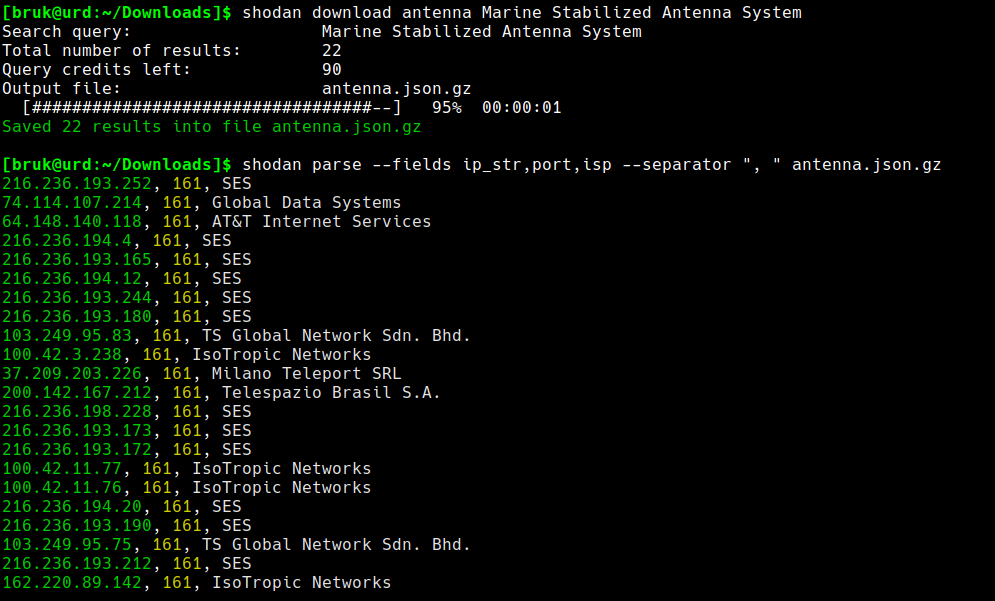
\includegraphics[scale=0.4]{Figurer/banner_parsing.png}
    \caption{Using the Shodan CLI to download and parse results. Results are listed with IP addresses, open ports and ISP.}
    \label{fig:banner_parsing}
\end{figure}

In the millions of devices connected to the internet, 22 devices is not really very many. However, this is the most accurate device identification this project was able to do. While the other approaches are also able to identify devices, it is not ceritan that those are a part of the offshore or maritime industries. The Cobham Seatel Satcom antenna is definetly a part of the navigation system of a ship, which is a maritime Cyber-Physical System. This one result was also one not found by this project, but by another project. More specifically, it was found by someone who has more insight into the industry, showing that device identification by banner specification is easier with experience from area of work within the constraints.

\subsection{ISP}
For identifying devices by looking at Internet Service Providers (ISP), DNV-GL suggested to look into Tampnet. On their webpage, the follwing can be found: "By providing a fast subsea fibre optic network and 4G LTE coverage, Tampnet enables digitalization of offshore operations within oil & gas, maritime and wind energy." \cite{tampnet} Tampnet is an ISP that provides internet connections to the maritime, offshore and wind energy industries. 
\todo[inline]{Finish this chapter}

\subsection{Reverse Geolocation}
\todo[inline]{Finish this chapter}

With many major seaports, like Rotterdam, Antwerp and Hamburg, the North Sea has a lot of marine traffic. The sea also has a lot of offshore oil and gas fields; Ekofisk, Sleipner, Forties and Valhall, to mention a few.\cite{oil_field_lists} With this much activity within both constraints, the marine and offshore industries, a lot of things in the area have to be connected to the internet. To test if the IP geolocation services of Shodan could detect devices connected to the internet, a large area of the North sea was chosen: a circle with 270 km around 56\degree24\textquotesingle00.0N 3\degree00\textquotesingle36.0E, as seen in \cref{fig:geolocation}. To use Shodan to find devices within this area, the command \cref{lst:geolocation_sea} was used. As seen in the output from the command, no devices was found within the area.

\begin{figure} [H]
    \centering
    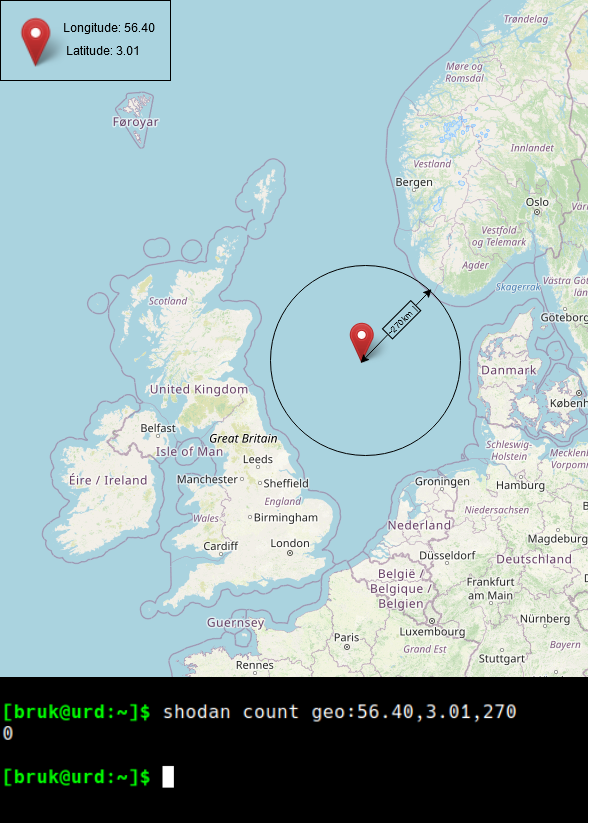
\includegraphics[scale=0.7]{Figurer/geolocation.png}
    \caption{Shodan "geo" filter visualized. Map copyright: https://www.openstreetmap.org/copyright}
    \label{fig:geolocation}
\end{figure}

\subsection{Latency and traceroute}
\todo[inline]{write this chapter}
\subsection{Problems}
\subsubsection{NAT}
Due to NAT connecting devices to the internet trough a single router, Shodan will only scan the outer NAT routing device, and not the devices behind the NAT. NAT is not always used for getting more IPv4 addresses. Sometimes it is used purposely to hide IPv4 addresses from the public internet.

\subsubsection{firewalls}
\todo[inline]{Maybe write this chapter}

\subsection{Combination of methods} \label{sec:combo}
\todo[inline]{Maybe write this chapter}
